
% This LaTeX was auto-generated from MATLAB code.
% To make changes, update the MATLAB code and republish this document.

\documentclass{article}
\usepackage{graphicx}
\usepackage{color}

\sloppy
\definecolor{lightgray}{gray}{0.5}
\setlength{\parindent}{0pt}

\begin{document}

    
    \begin{verbatim}
clear;close all;clc;
\end{verbatim}
\begin{par}
Exact model
\end{par} \vspace{1em}
\begin{verbatim}
% Continuous time Butterworth filter
% Filter order : 1
% Cutoff angular frequency : [0.01,0.2]

[B_tilde,A_tilde] = butter(1,[0.01,0.2],'s');

B_tilde = B_tilde/A_tilde(3);
A_tilde = A_tilde/A_tilde(3);

w_start = 0.001;
w_stop = 2;

N = 500;            % Number of frequencies

W = linspace(w_start,w_stop,N)';

% Exact frequency response of the reference filter
G_0 = freqs(B_tilde,A_tilde,W);
% freqs(B_tilde,A_tilde,N)

% Circular zero mean white noise
sigma = 0.001;          % Standard deviation
noise = sigma*(randn(N,1) + 1i*randn(N,1))/sqrt(2);

% Measured frequncy response
G_m = G_0 + noise;

% Rewrite the transfer funciton
s = 1i*W;
s_all = s.^((0:length(B_tilde)-1));
s_all = fliplr(s_all);
\end{verbatim}
\begin{verbatim}
B_true = polyval(B_tilde,s);
\end{verbatim}
\begin{verbatim}
A_prime_true = polyval([A_tilde(1:2) 0],s);

% True parameters
% theta_true = [A_tilde(2:3) B_tilde(1:3)];
% theta_true = fliplr(theta_true).';

theta_true = [B_tilde(1:3) A_tilde(1:2)];
theta_true = (theta_true).';

% Plots
% figure;
% Wlog = logspace(-3,1,N);
% loglog(Wlog,abs(G_0));
% hold on;
% loglog(Wlog,abs(G_m));
% grid on;
% legend('Exact frequency response','Measured frequncy response')
% xlabel('Frequency (rad/s)');
% ylabel('Magnitude');
%
% figure;
% plot(W,db(G_0));
% hold on;
% plot(W,db(G_m));
% grid on;
% legend('Exact frequency response','Measured frequncy response');
\end{verbatim}

\begin{verbatim}Implemenation of the Levy estimators\end{verbatim}
    \begin{verbatim}
% Cost function vectorization
e_Levy = G_m ;

% Jacobian
J_Levy = [-s_all(:,1) -s_all(:,2) -s_all(:,3) G_m.*s_all(:,1) G_m.*s_all(:,2)];

% Real/imaginary part separation
e_Levy_IR = [real(e_Levy) ; imag(e_Levy)];
J_Levy_IR = [real(J_Levy) ; imag(J_Levy)];

% Levy theta estimation
theta_Levy = -J_Levy_IR\e_Levy_IR;

GestLevy = freqs(theta_Levy(1:3),[theta_Levy(4:5); 1],W);
\end{verbatim}
\begin{verbatim}
figure
plot(W,db(GestLevy),'o',W,db(G_m),'*',W,db(G_0),'+')
xlabel('Freq [rad]');
ylabel('Magn [dB]');

Bias = G_0 - GestLevy;
figure('Name','Levy estimation')
semilogx(W,db(GestLevy),W,db(G_m),'*',W,db(e_Levy),'+',W,db(sigma*ones(N,1)),W,db(Bias))
legend('Levy estimation','G_m','e_{LS}','\sigma_{means}','Bias')
xlabel('Freq [rad]');
ylabel('Magn [dB]');

disp('Parameters comparison');
disp(join(['True theta:           ',num2str(theta_true.')]));
disp(join(['Levy estimated theta: ',num2str(theta_Levy(1:end).')]));
% disp(join(['Difference:           ',num2str(theta_true.' - theta_Levy(1:end-1).')]));
\end{verbatim}

        \color{lightgray} \begin{verbatim}Parameters comparison
True theta:           0   95    0  500   95
Levy estimated theta: 0.0080435      1.0349     0.92247       5.497      5.7842
\end{verbatim} \color{black}
    
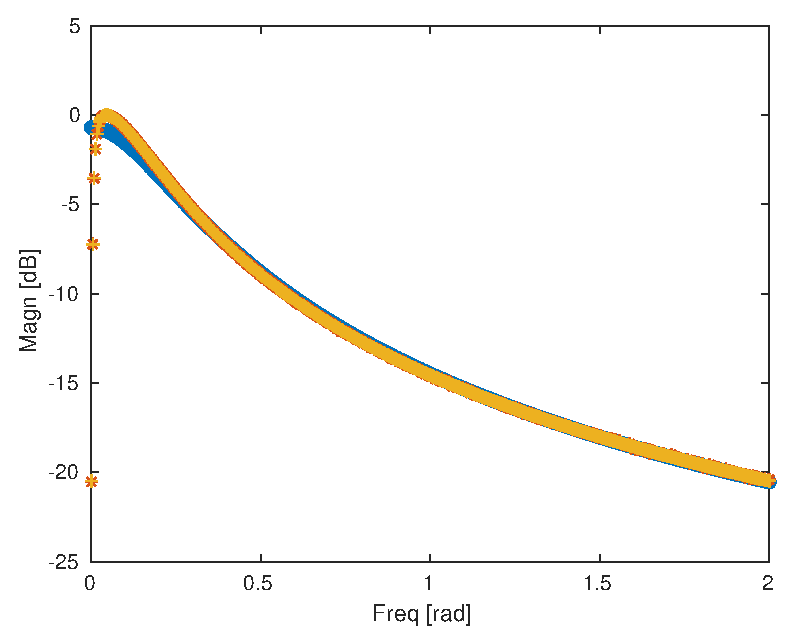
\includegraphics [width=4in]{main_01.eps}

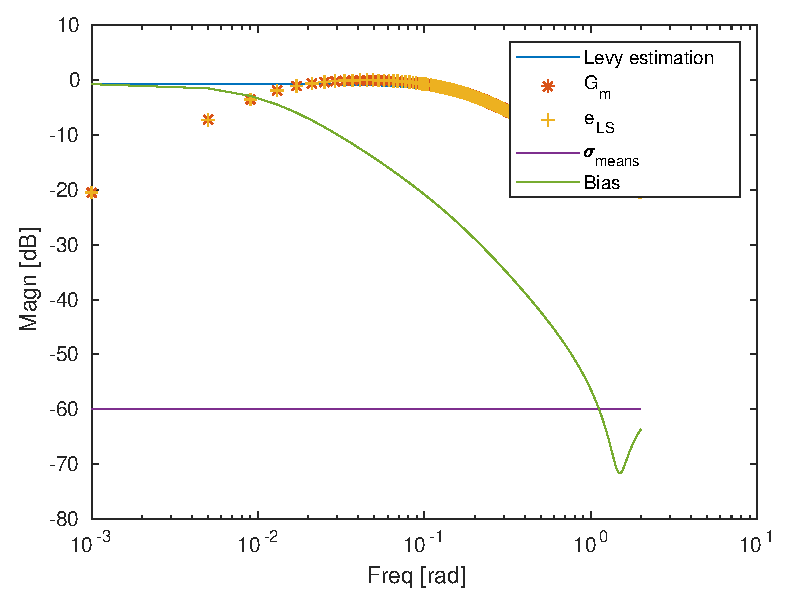
\includegraphics [width=4in]{main_02.eps}

\begin{verbatim}Implemenation of the Sanathanan estimator\end{verbatim}
    \begin{verbatim}
% Iteration index
l_San_max = 20;

% Computing B with new parameters
B = polyval(theta_Levy(1:3),s);

% Computing A with new parameters
A_prime = zeros(N,1);

% Cost function vectorization
e_San = G_m;

% Jacobian
J_San = J_Levy;

% Real/imaginary part separation
e_San_IR = [real(e_San) ; imag(e_San)];
J_San_IR = [real(J_San);imag(J_San)];

theta_San = zeros(5,1);

% Sanathanan estimation
for l = 1:l_San_max

    % Parameters computation
    theta_San = -J_San_IR\e_San_IR;

    % Computing B with new parameters
    B = polyval(theta_San(1:3).',s);

    % Computing A with new parameters
    A_prime_new = polyval([theta_San(4:5).' 0],s);

    % Updating the cost function and the Jacobian
    e_San = G_m ./vecnorm(1+A_prime,2,2);
    J_San = J_Levy./vecnorm(1+A_prime,2,2);

    e_San_IR = [real(e_San) ; imag(e_San)];
    J_San_IR = [real(J_San) ; imag(J_San)];

    % Saving the previous A_prime
    A_prime = A_prime_new;
end

GestSan = freqs(theta_San(1:3),[theta_San(4:5); 1],W);
\end{verbatim}
\begin{verbatim}
figure('Name','Sanathanan estimation')
plot(W,db(GestSan),'o',W,db(G_m),'*',W,db(G_0),'+')
legend('Sanathanan','G_m','G_0')
xlabel('Freq [rad]');
ylabel('Magn [dB]');

Bias = G_0 - GestSan;
figure('Name','Sanathanan estimation')
semilogx(W,db(GestSan),W,db(G_m),'*',W,db(e_San),'+',W,db(sigma*ones(N,1)),W,db(Bias))
legend('Sanathanan estimation','G_m','e_{LS}','\sigma_{means}','Bias')
xlabel('Freq [rad]');
ylabel('Magn [dB]');


disp(join(['Sanathanan estimated theta: ',num2str(theta_San.')]));
\end{verbatim}

        \color{lightgray} \begin{verbatim}Sanathanan estimated theta: 0.0125695      94.99906  0.0003299869      499.9279       95.0072
\end{verbatim} \color{black}
    
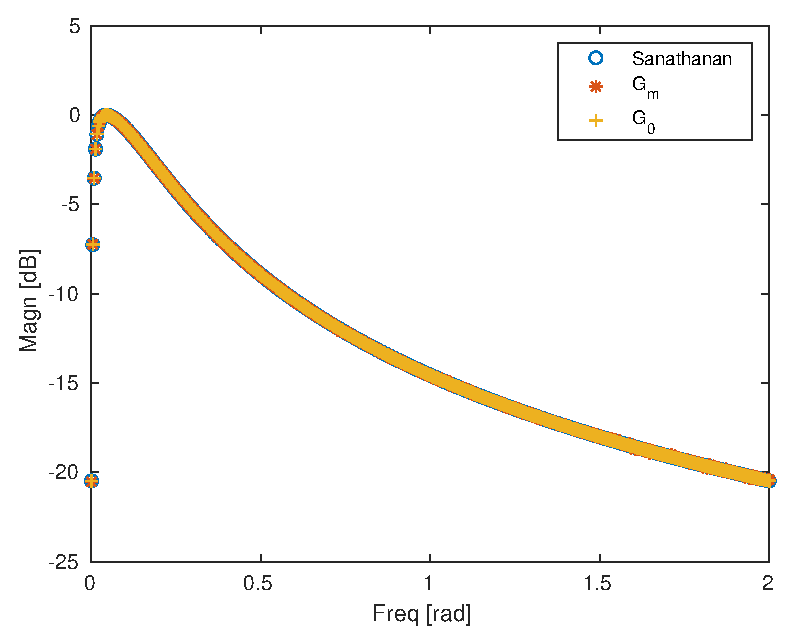
\includegraphics [width=4in]{main_03.eps}

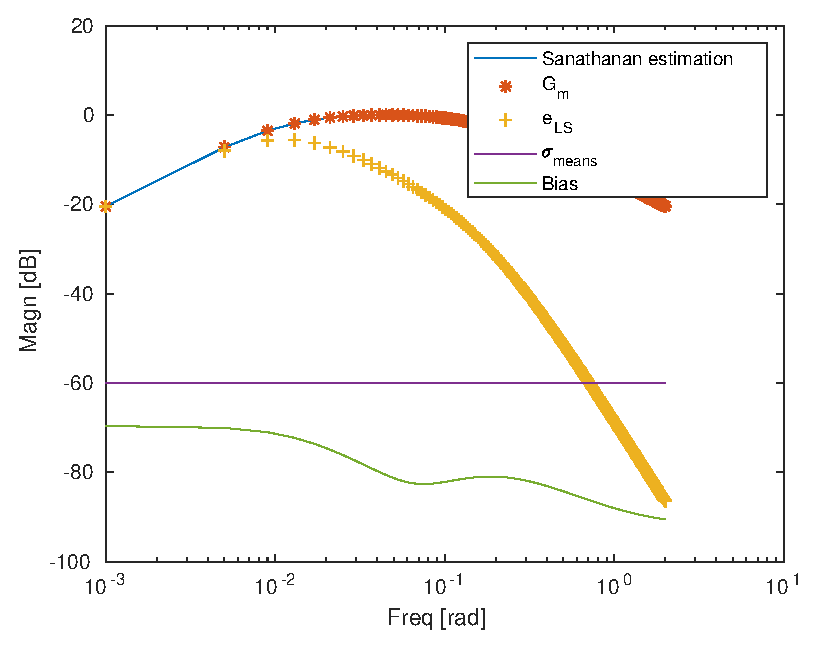
\includegraphics [width=4in]{main_04.eps}

\begin{verbatim}Implemenating Gauss-Newton based least squares estimation\end{verbatim}
    \begin{verbatim}
% Initial parameters
theta_GN = theta_Levy;

% Number of iterations
l_GN_max = 20;

for l = 1:l_GN_max

    % Computing B with new parameters
    B = polyval(theta_GN(1:3).',s);

    % Computing A with new parameters
    A = polyval([theta_GN(4:5).' 1],s);

    % Cost function
    e_GN = G_m - B./A;

    % Jacobian
    J_GN = [-s_all(:,1) -s_all(:,2) -s_all(:,3) B.*s_all(:,1)./A B.*s_all(:,2)./A]./A;

    % Real values matrices
    e_GN_IR = [real(e_GN) ; imag(e_GN)];
    J_GN_IR = [real(J_GN) ; imag(J_GN)];

    % Delta theta
    delta_theta = -J_GN_IR\e_GN_IR;

    % Theta(l+1) = theta(l) + delta_theta
    theta_GN = theta_GN + delta_theta;

end

GestGN = freqs(theta_GN(1:3),[theta_GN(4:5); 1],W);
\end{verbatim}
\begin{verbatim}
figure('Name','Maximum likelihood estimation')
plot(W,db(GestGN),'o',W,db(G_m),'*',W,db(G_0),'+')
legend('Maximum likelihood estimation','G_m','G_0')
xlabel('Freq [rad]');
ylabel('Magn [dB]');

Bias = G_0 - GestGN;
figure('Name','Maximum likelihood estimation')
semilogx(W,db(GestGN),W,db(G_m),'*',W,db(e_GN),'+',W,db(sigma*ones(N,1)),W,db(Bias))
legend('Maximum likelihood','G_m','e_{LS}','\sigma_{means}','Bias')
xlabel('Freq [rad]');
ylabel('Magn [dB]');
\end{verbatim}

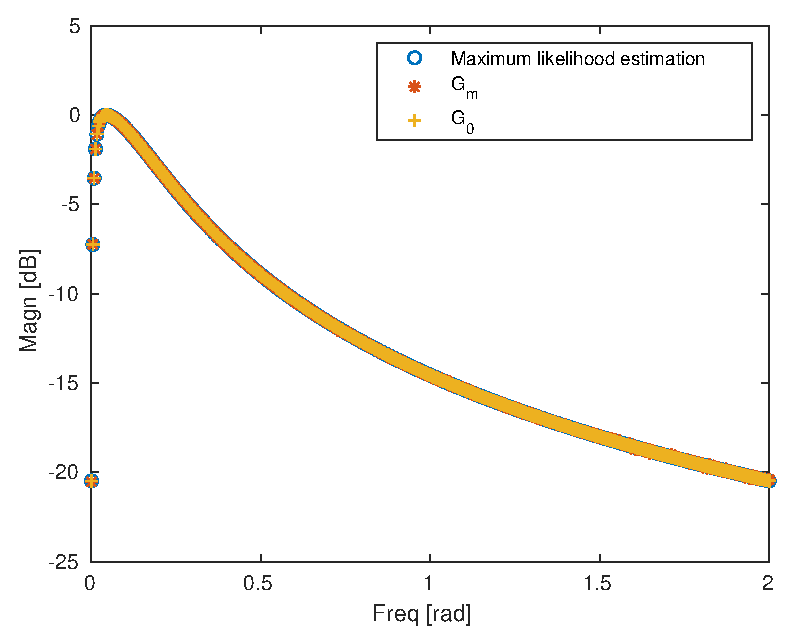
\includegraphics [width=4in]{main_05.eps}

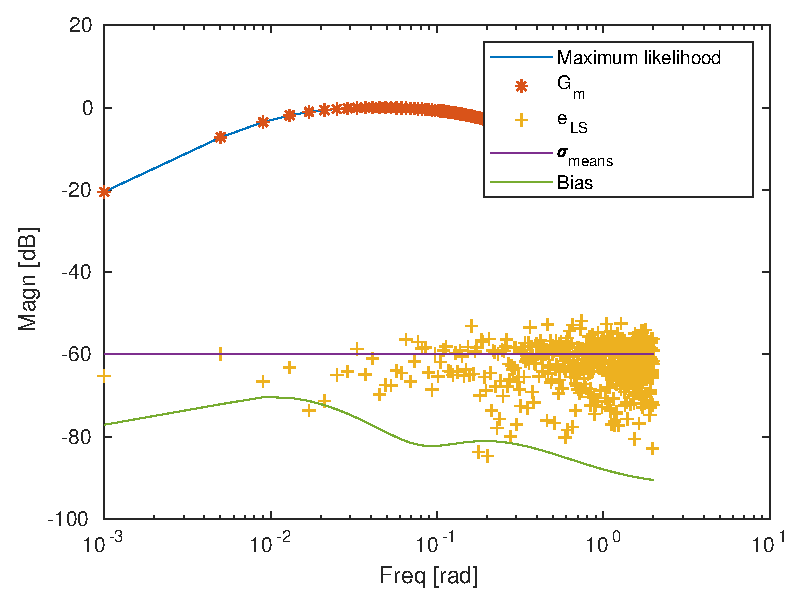
\includegraphics [width=4in]{main_06.eps}



\end{document}
    
